\chapter{Architectural Overview}
\label{ch:architectural_overview}
In this chapter, the architectural overview of the run-time state migration approach is discussed. First, the publish-subscribe pattern is explained as a mean to exchange state information and manage available devices as well as which state models are supported by an application. The middleware is explained next, which uses the publish-subscribe pattern and acts as a message broker. Subsequently, the library as well as the interfaces that need to be implemented by the respective applications are explained. The last part explains the message exchange in the different life cycle phases of the migration approach.

\section{Publish–subscribe pattern}
An infrastructure is needed to exchange run-time states of applications across different devices. Also, devices should know which other devices with common Application State Models are available and notice if they join or leave the network. Moreover, devices should be able to migrate the run-time state and acknowledge other devices when migration is done.

In this approach, we chose to use the publish-subscribe pattern. Thereby, the middleware is the message broker, devices are publishers and subscribers, Application State Models are topics, and run-time states are messages. Also, there are extra topics and messages that allow us to fulfil requirements such as device introduction, device connectivity and finalizing the run-time state migration.

Figure \ref{fig:publish–subscribe} illustrates an overview of publish–subscribe pattern in our approach. A Mac device (see \fcircone) subscribes to \textit{Model-A} and \textit{Model-B} topics, a Windows device (see \fcirctwo) subscribes to \textit{Model-A} topic and an Android device (see \fcircthree) subscribes to \textit{Model-B} topic. The Mac device publishes a message contain \textit{"X"} to topic \textit{Model-A}, and the middleware makes sure it gets forwarded to the Windows device. Also, a message containing \textit{"Y"} is published from the Mac device to the topic \textit{Model-B} and forwarded to the Android device by the middleware.

\vspace{10mm}
\FloatBarrier \begin{figure}[H]
    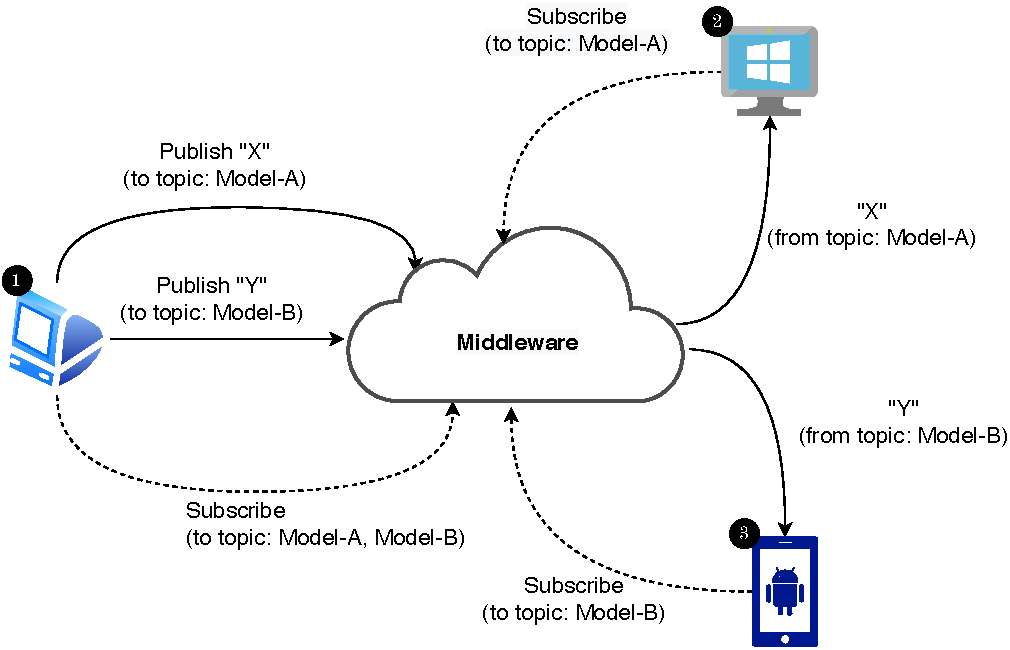
\includegraphics[width=0.8\textwidth]{../figures/publish-subscribe.pdf}
    \centering
    \caption{Overview of Publish–subscribe pattern in our approach.}
    \label{fig:publish–subscribe}
\end{figure} \FloatBarrier

\subsection{Middleware}
As middleware acts as a message broker, if devices are not on the same network, a middleware should exist in which applications can communicate with each other. Figure \ref{fig:solution-overview} shows the role of middle-ware.
This middleware can handle sending and receiving the run-time state.
The goal of having this middleware is applications which coupled with
libraries, can introduce themselves, find each other, and migrate the run-time state.

Also, as mentioned in \textbf{R4 Device Management}, middleware is responsible for device discovery and notifying other devices if a device joins or leaves with the same Application State Model. The message exchange for device discovery is explains in subchapter 6.5.

As in this thesis, we considered the publish-subscribe pattern as the architecture, middleware is the intermediary message broker.

\subsection{Topics}
There are some topics each device should subscribe to them. Devices who subscribed to these topics receive a message if another device publish a message to them.

\subsubsection{Topic for Connectivity Status}
All devices should subscribe to a topic about their connectivity status. This topic is \lstinline[basicstyle=\ttfamily]{online}. If a device joins or leaves the network, other devices get notice by a message.

\subsubsection{Topics for Application State Models}
Each Application State Model has a topic. Devices that supports these Application State Models should subscribe to these topics. So, if a device joins the same topic, it should notify other devices about joining and supporting the same Application State Model and also other devices notify the new device about their existence as a response. Moreover, for each Application State Model, devices should subscribe to the subtopic of device identification, that they can receive an individual message from other devices and vice versa. As users may use different devices and applications device identification must be unique like UUID; to improve the readability of the following example, we use a combination of the operating system and application name as the UUID. Of course, the is only done for the examples in the thesis and would lead to name clashes in a broader scenario. In a live setting, the UUID would be randomly generated.



\subsubsection{Example Scenario}
Considering the scenario of Figure \ref{fig:asml-overview}. Three devices share some Application State Models. All devices should subscribe to \lstinline[basicstyle=\ttfamily]{online} topic. Mailspring supports three Application State Models, so it should subscribe to topics:
\begin{verbatim}
online
search
new-event
sending-email
\end{verbatim}

Also, to guarantee that other devices on the same topic can send message to Mailspring, it should subscribe to these subtopics with its identification: 
\begin{verbatim}
search/mac-mailspring
new-event/mac-mailspring
sending-email/mac-mailspring
\end{verbatim}

As K-9 Mail supports two Application State Models, it has to subscribe to these topics:
\begin{verbatim}
online
search
sending-email
search/android-k9mail
sending-email/android-k9mail
\end{verbatim}


Also, as Woven supporting one Application State Model, it has to subscribe to these topics:
\begin{verbatim}
online
new-event
new-event/windows-woven
\end{verbatim}

% So, if K-9 Mail and Woven are already in the network and Mailspring joins, it  sends a message to topics \lstinline[basicstyle=\ttfamily]{search}, \lstinline[basicstyle=\ttfamily]{sending-email} and \lstinline[basicstyle=\ttfamily]{new-event} which allows K-9 Mail and Woven get notify about joining the new device with common Application State Models. Also, Woven sends back a introduction response message to \lstinline[basicstyle=\ttfamily]{new-event/mac-mailspring} about its existence. Morever, K-9 Mail should do the same but to \lstinline[basicstyle=\ttfamily]{search/mac-mailspring} and \lstinline[basicstyle=\ttfamily]{sending-email/mac-mailspring} topics.


\subsection{Messages}
In this architecture, we need some message to fulfill our requirements like device introduction.

\subsubsection{Device Introduction}
When a user runs an application, the application should introduce itself to other devices on the network. Moreover, other devices should get notify and response with their introduction.

\subsubsection{Device Leave}
After an application got closed or a device went offline, it should notify other devices about this message. Moreover, other devices should not be able to communicate with that device.

\subsubsection{Device Has Run-time State}
If a device has a run-time state, it should notify other devices which support  common Application State Model.

\subsubsection{Request Run-time State}
A device can request a run-time state of other devices supporting the common Application State Model. The target device should respond to this request.

\subsubsection{Send Run-time State}
As the source device can request a run-time state, the target device should respond to this request by sending its run-time state. Also, the source application should be aware of receiving it.

\subsubsection{Run-time State Migration}
After the target device received a run-time state and is adjusted into the application, the target device should notify the source device about finalizing the run-time state migration to react to this message.

\subsection{Actions}
In this architecture, we need some actions to fulfill our requirements like store a run-time state.

\subsubsection{Store Run-time State}
If a device has a run-time state, it should be stored if other devices request the run-time state migration.

\subsubsection{Add Device}
If a device gets a Device Introduction message, it should add that particular device to its list.

\subsubsection{Remove Device}
If a device gets a Device Leave message, it should remove that particular device from its list.

\section{Library}
As state in \textbf{R1 Applicable on Existing Applications}, this approach is meant to support run-time state migration for existing applications on different platforms; special libraries in different programming languages and platforms should be developed. 
These libraries should provide basic functionality such as communication, validation of run-time states based on an Application State Model, and an API to support extraction and injection of run-time states between same-purpose applications with common Application State Model.

Developers can integrate these libraries in existing applications to enable run-time state migration, and they should implement some glue code in existing source code to adapt the library into existing applications (Figure \ref{fig:solution-overview}).

The library reflect are the generic part of run-time state migration, the glue code and the interfaces derived from the application state model reflect the application specific part.

These libraries should be written in the same programming languages as the source and target applications. These libraries should be able to communicate directly or with the help of middleware.
If devices are on the same local network, these libraries should establish a point-to-point connection.
Otherwise, they should be able to communicate with help the middleware over the internet.
In this case, they should introduce themselves to the middleware to find each other; then, they can migrate the run-time state.


\section{Interfaces}
Interfaces are derived from Application State Model, and they guarantee certain values on a run-time state. They can be auto-generated or manually written by developers with same programming language of the source and target applications.
To integrate the libraries into source code, developers should implement some glue code and use the interfaces like Figure \ref{fig:solution-overview}. Developers should add interfaces to the library with glue code. Thereby, the library will know which Application State Models has to be supported.

Considering Mailspring written in TypeScript, Listing \ref{lis:search-interface} shows a generated interface based on search Application State Model (Listing \ref{lis:search-schema}).

\FloatBarrier
\begin{code}
\begin{js}
export interface SearchObject {
    /**
     * the query of search
     */
    query: string;
    /**
     * shows if the query is already has been submitted
     */
    submit?: boolean;
}
\end{js}
\caption{Note Writing example interface in TypeScript.}
\label{lis:search-interface}
\end{code}
\FloatBarrier


\section{Life Cycles}
After explanation of entities of the architecture in previous sections, the interaction between these entities in different life cycle phases is explained. These life cycles phases consist of main entities, actions and sequence of messages discussed in the messages section, and they are implemented in chapter \ref{ch:implementation}. 
\subsection{Initializing}
After the user runs an application, an initialization step should happen to introduce itself to the other applications. This step uses the Device Introduction event. Figure \ref{fig:Initializing} shows a source application that joins the network and introduces itself with a message to library. Library publishes this message to all supported topics of Application State Models, and middleware forwards it to the library of the target application which subscribed to the same topic. Thereby, the library add the new device to a device list and notifies the target application about a new device. In response, target application introduce itself in the same way to the source application.



\FloatBarrier \begin{figure}[H]
    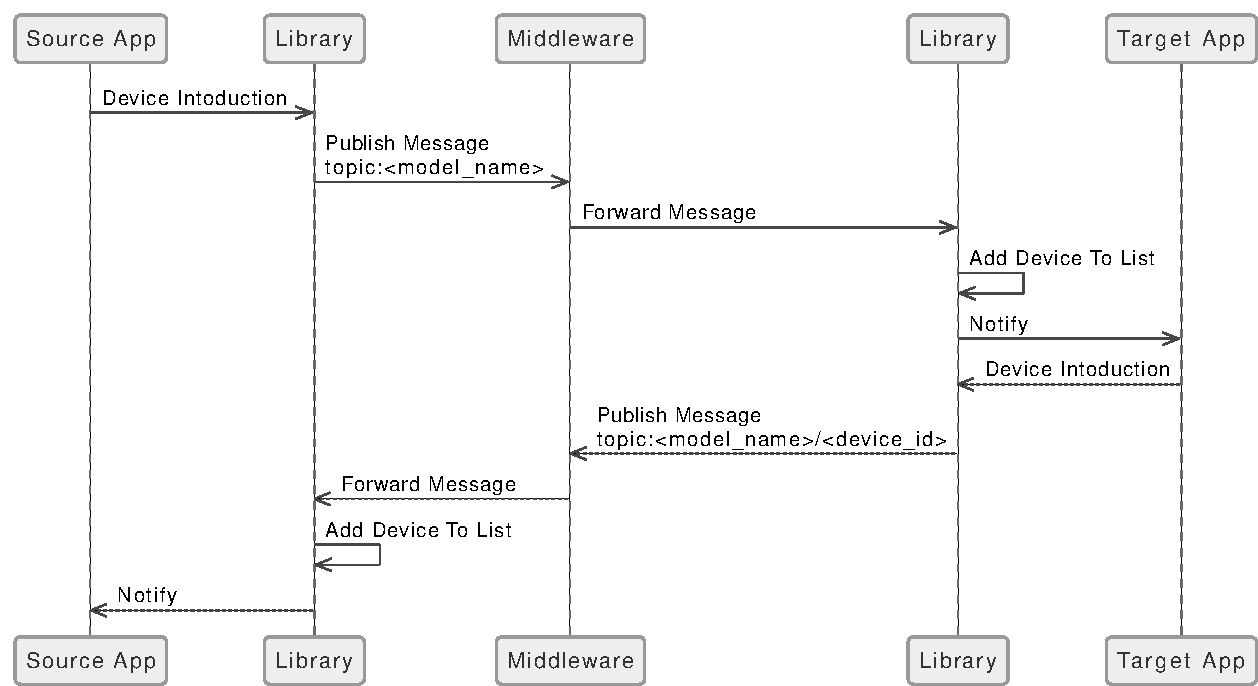
\includegraphics[width=\linewidth]{../figures/Initializing.pdf}
    \centering
    \caption{Initializing the Source Application}
    \label{fig:Initializing}
\end{figure} \FloatBarrier

\subsection{Going Offline}
An application might go offline by a user or even by other causes. A plan should cover these incidents. This step uses the Device Leave event. After disconnection, other devices are not allowed to send any message to that particular device.

\subsubsection{Graceful}
A user might close the application. In this case, the application goes offline gracefully, and it should notify other applications about its absence. Figure \ref{fig:Going-Offline-Graceful-Source} shows the source application going offline gracefully. With the library's help, the source application informs its absence to middleware on \lstinline[basicstyle=\ttfamily]{online} topic, and middleware forwards it to the library of the target application. Thereby, the library removes the device from devices list and notifies the target application about the leaving of the source application. 

\FloatBarrier \begin{figure}[H]
    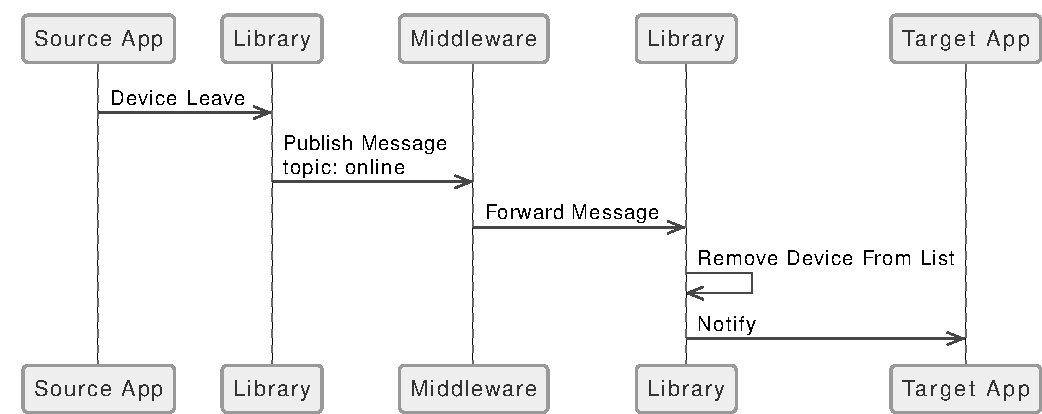
\includegraphics[width=\linewidth]{../figures/Going-Offline-Graceful-Source.pdf}
    \centering
    \caption{Going Offline Gracefully: Source}
    \label{fig:Going-Offline-Graceful-Source}
\end{figure} \FloatBarrier

\subsubsection{Ungraceful}
An application might go offline by other causes like network problems, device crashing, application failure, etc. In this case, the application goes offline ungracefully, and it should notify other applications about its absence. Figure \ref{fig:Going-Offline-Ungraceful-Source} shows the source application going offline ungracefully. The middleware checks if the application is connected; if it does not get any response, request gets a timeout and it publishes a message to  \lstinline[basicstyle=\ttfamily]{online} topic. Thereby, the library removes the device from devices list notifies the target application about the leaving of the source application.

\FloatBarrier \begin{figure}[H]
    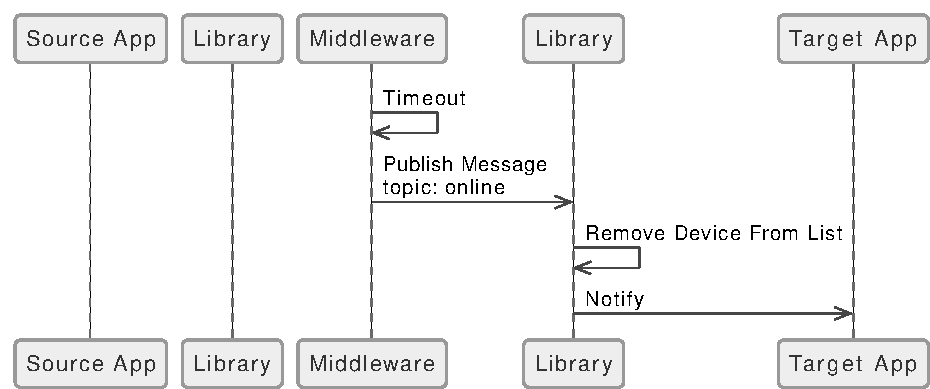
\includegraphics[width=\linewidth]{../figures/Going-Offline-Ungraceful-Source.pdf}
    \centering
    \caption{Going Offline Ungracefully: Source}
    \label{fig:Going-Offline-Ungraceful-Source}
\end{figure} \FloatBarrier

\subsubsection{Has Run-Time State}
To migrate a run-time state, an application should have a run-time state. Any application with a run-time state should notify other applications about it if they request a run-time state. This step uses the Device Has State event. Figure \ref{fig:Inform-Devices-Has-State-Source} shows the source application has a run-time state and informs the middleware by publish a message to topics of Application State Models and middleware forward it to the library of the target application. Thereby, the library notifies the target application about the source application, which has a run-time state.

\FloatBarrier \begin{figure}[H]
    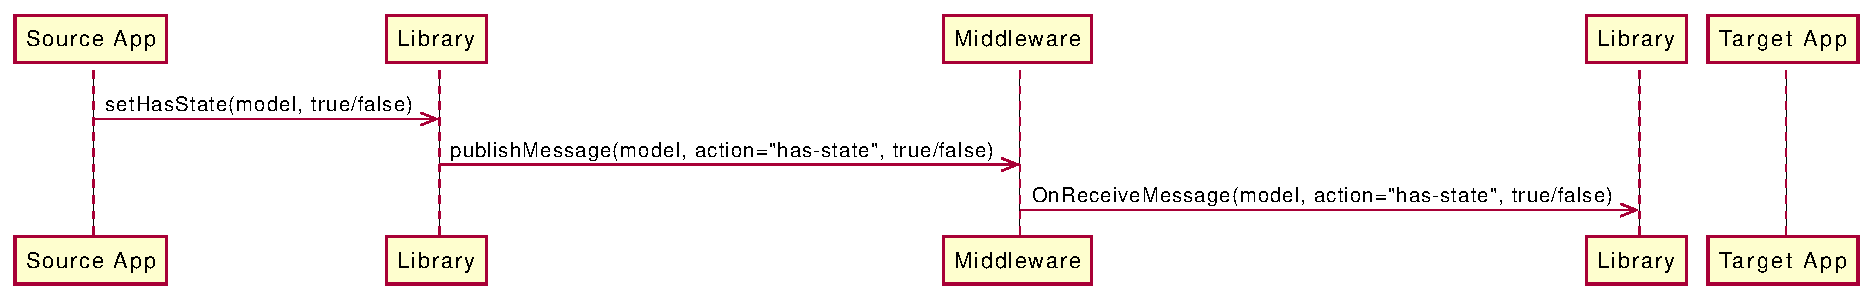
\includegraphics[width=\linewidth]{../figures/Inform-Devices-Has-State-Source.pdf}
    \centering
    \caption{Source App inform other devices that has a state}
    \label{fig:Inform-Devices-Has-State-Source}
\end{figure} \FloatBarrier

\subsection{Store Run-time State}
To migrate a run-time state of an application, it should be temporarily stored and ready for migration if other applications request it. Figure \ref{fig:Store-Current-State} shows that the source and target applications can temporarily store their run-time state in the library.

\FloatBarrier \begin{figure}[H]
    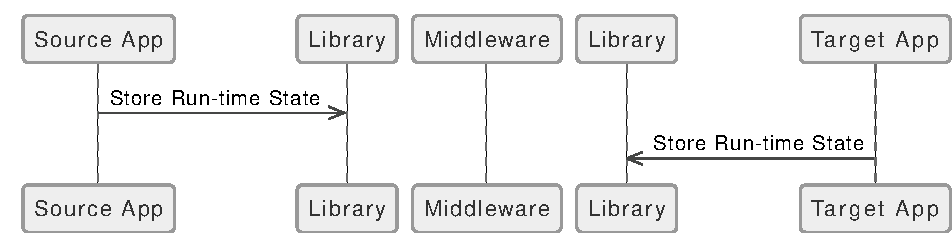
\includegraphics[width=\linewidth]{../figures/Store-Current-State.pdf}
    \centering
    \caption{Store the Current State}
    \label{fig:Store-Current-State}
\end{figure} \FloatBarrier


\subsection{Migration Patterns}
In this section, we describe two patterns for run-time state migration.

\subsubsection{Pull Method}
In the pull method, source applications request a run-time state from the target application. Figure \ref{fig:Migration-Source-to-Target-Pull-Method} shows the source application gets the list of devices with a common Application State Model, then selects the target application and requests its run-time state by sending a message from the library to middleware. The middleware forwards the message, and the target application gets a request of its run-time state. After processing the request, the target application sends its run-time state by the library to middleware. The middleware forwards the message, and the source application receives the run-time state. Source application adjusts the new run-time state and notifies the target application about finalizing the run-time state migration by sending a message to the library and middleware. 

\FloatBarrier \begin{figure}[H]
    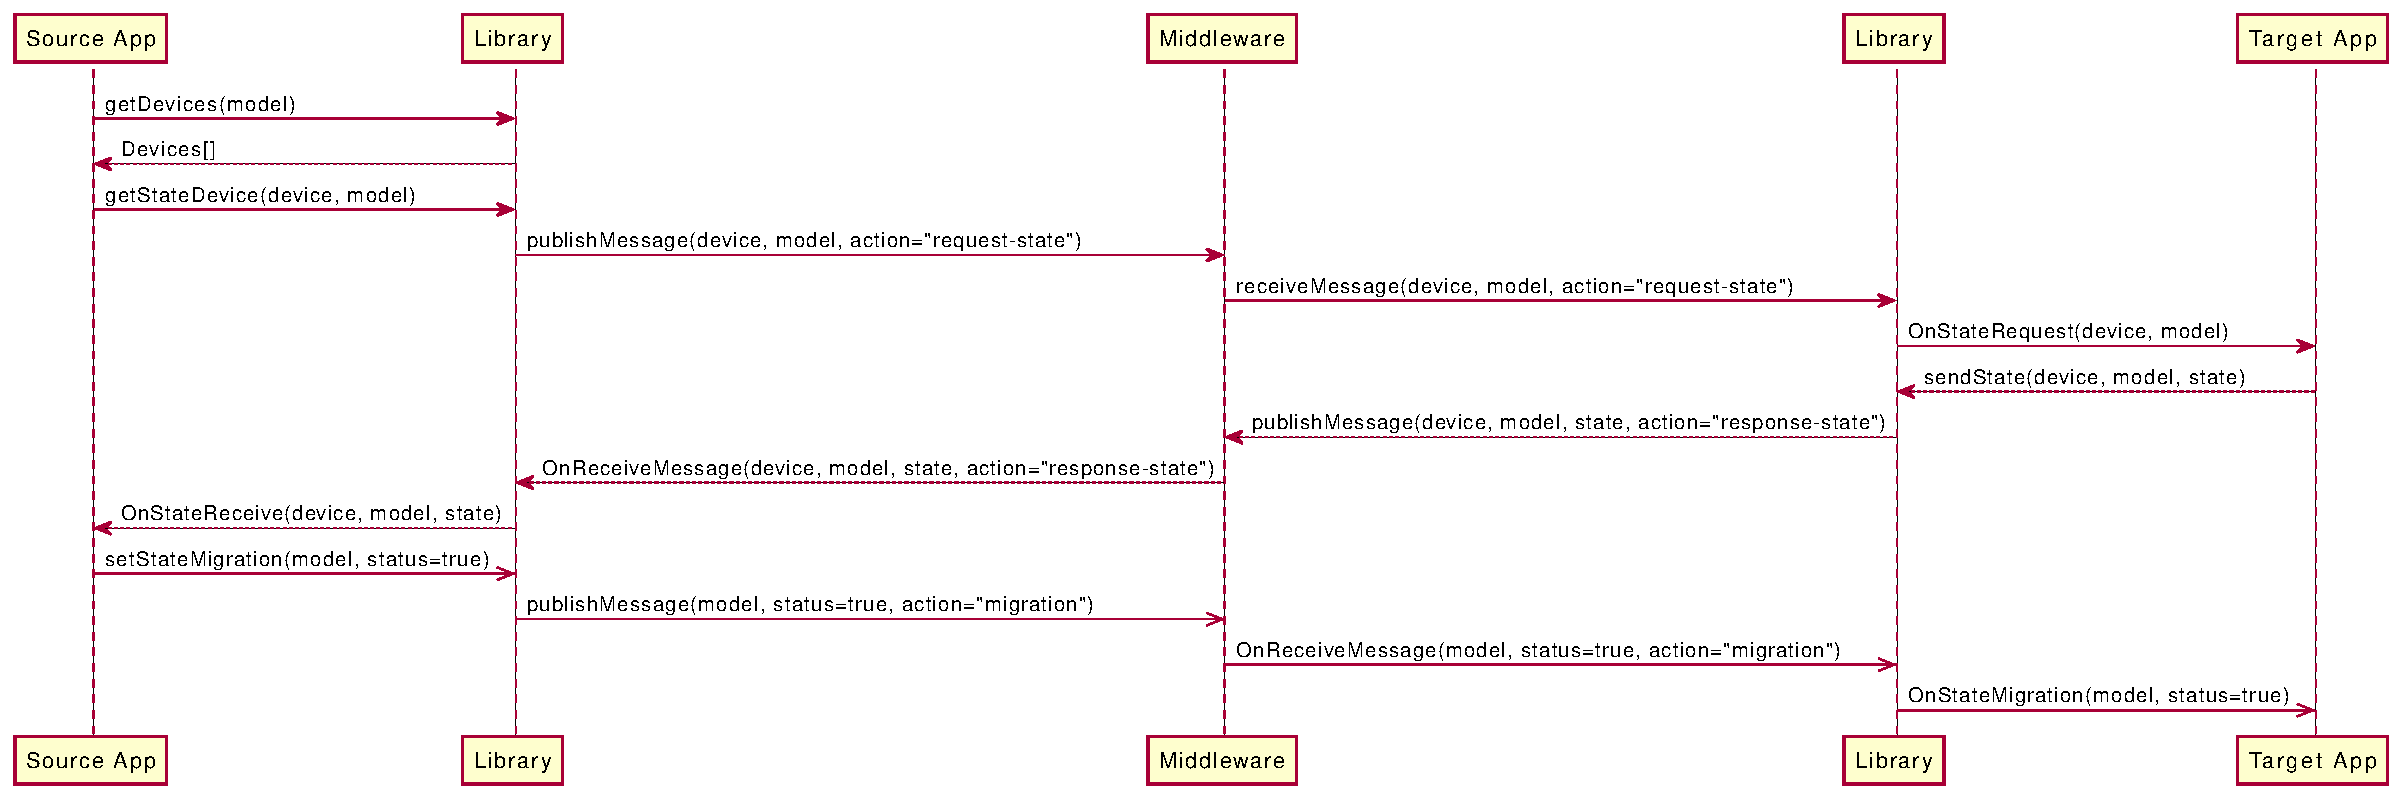
\includegraphics[width=\linewidth]{../figures/Migration-Source-to-Target-Pull-Method.pdf}
    \centering
    \caption{Pull Method: Migration Source to Target}
    \label{fig:Migration-Source-to-Target-Pull-Method}
\end{figure} \FloatBarrier

\subsubsection{Push Method}
In the push method, source applications send their run-time state to the target application without a request by force. Figure \ref{fig:Migration-Source-to-Target-Push-Method} shows the source application gets the list of devices with a common Application State Model, then selects the target application and requests its run-time state by sending a message from the library to middleware. The middleware forwards the message, and the target application gets a request of its state. After processing the request, the target application sends its run-time state by the library to middleware. The middleware forwards the message, and the source application receives the run-time state. Source application adjusts the new run-time state and notifies the target application about finalizing the run-time state migration by sending a message to the library and middleware. 

\FloatBarrier \begin{figure}[H]
    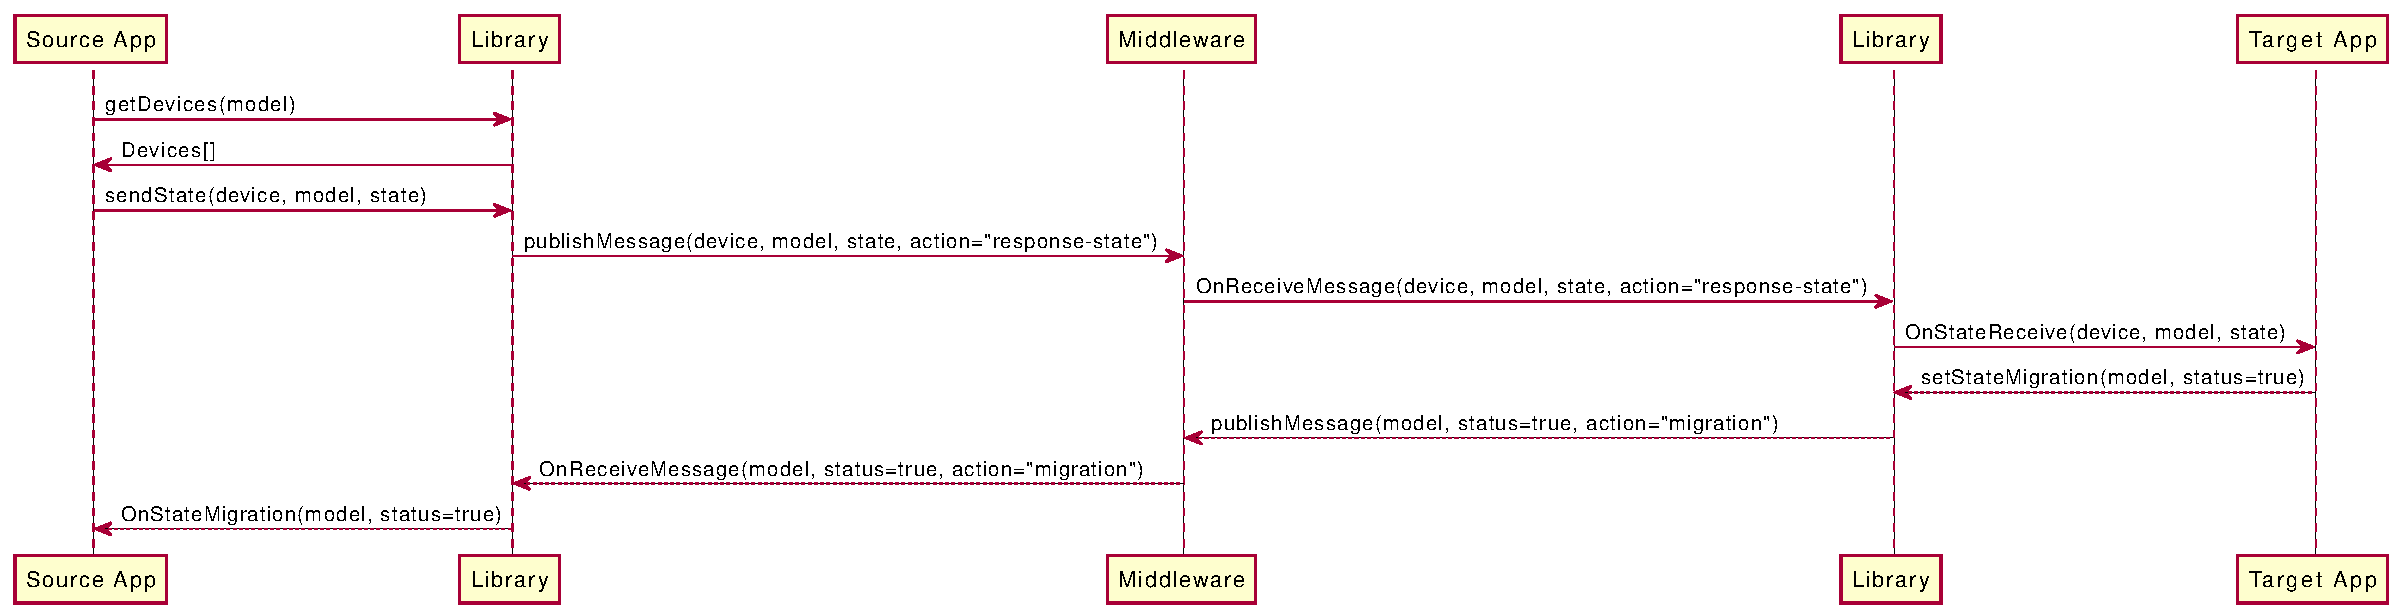
\includegraphics[width=\linewidth]{../figures/Migration-Source-to-Target-Push-Method.pdf}
    \centering
    \caption{Push Method: Migration Source to Target}
    \label{fig:Migration-Source-to-Target-Push-Method}
\end{figure} \FloatBarrier




\section{Model Repository}

As stated in requirement \textbf{R3 Model Repository}, we made a repository manager call Model Repository located on GitHub\footnote{\url{https://github.com/asml-lang/model-repository}}. Some models are available on this repository. Developers may use the search ability of GitHub to find their models. Also, after making a new model, developers can add it the repository manager by making a pull request. So, other developers may use it for their applications.

Currently, a GitHub repository is sufficient for this thesis. Although conceptually, we may be able to improve the Model Repository so that developers may easily search the model they need by name, description, or keywords and download or customize them. In addition, if the developer does not find the model they need, they could create a custom model using the Model Repository editor. Additionally, the models may be uploaded to the Model Repository if they have already developed one. The concept behind the solution is valid; however, implementation is a future work objective. Figure \ref{fig:model-repo} is an improved Model Repository that shown as a wireframe concept.

\FloatBarrier
\begin{figure}[H]
    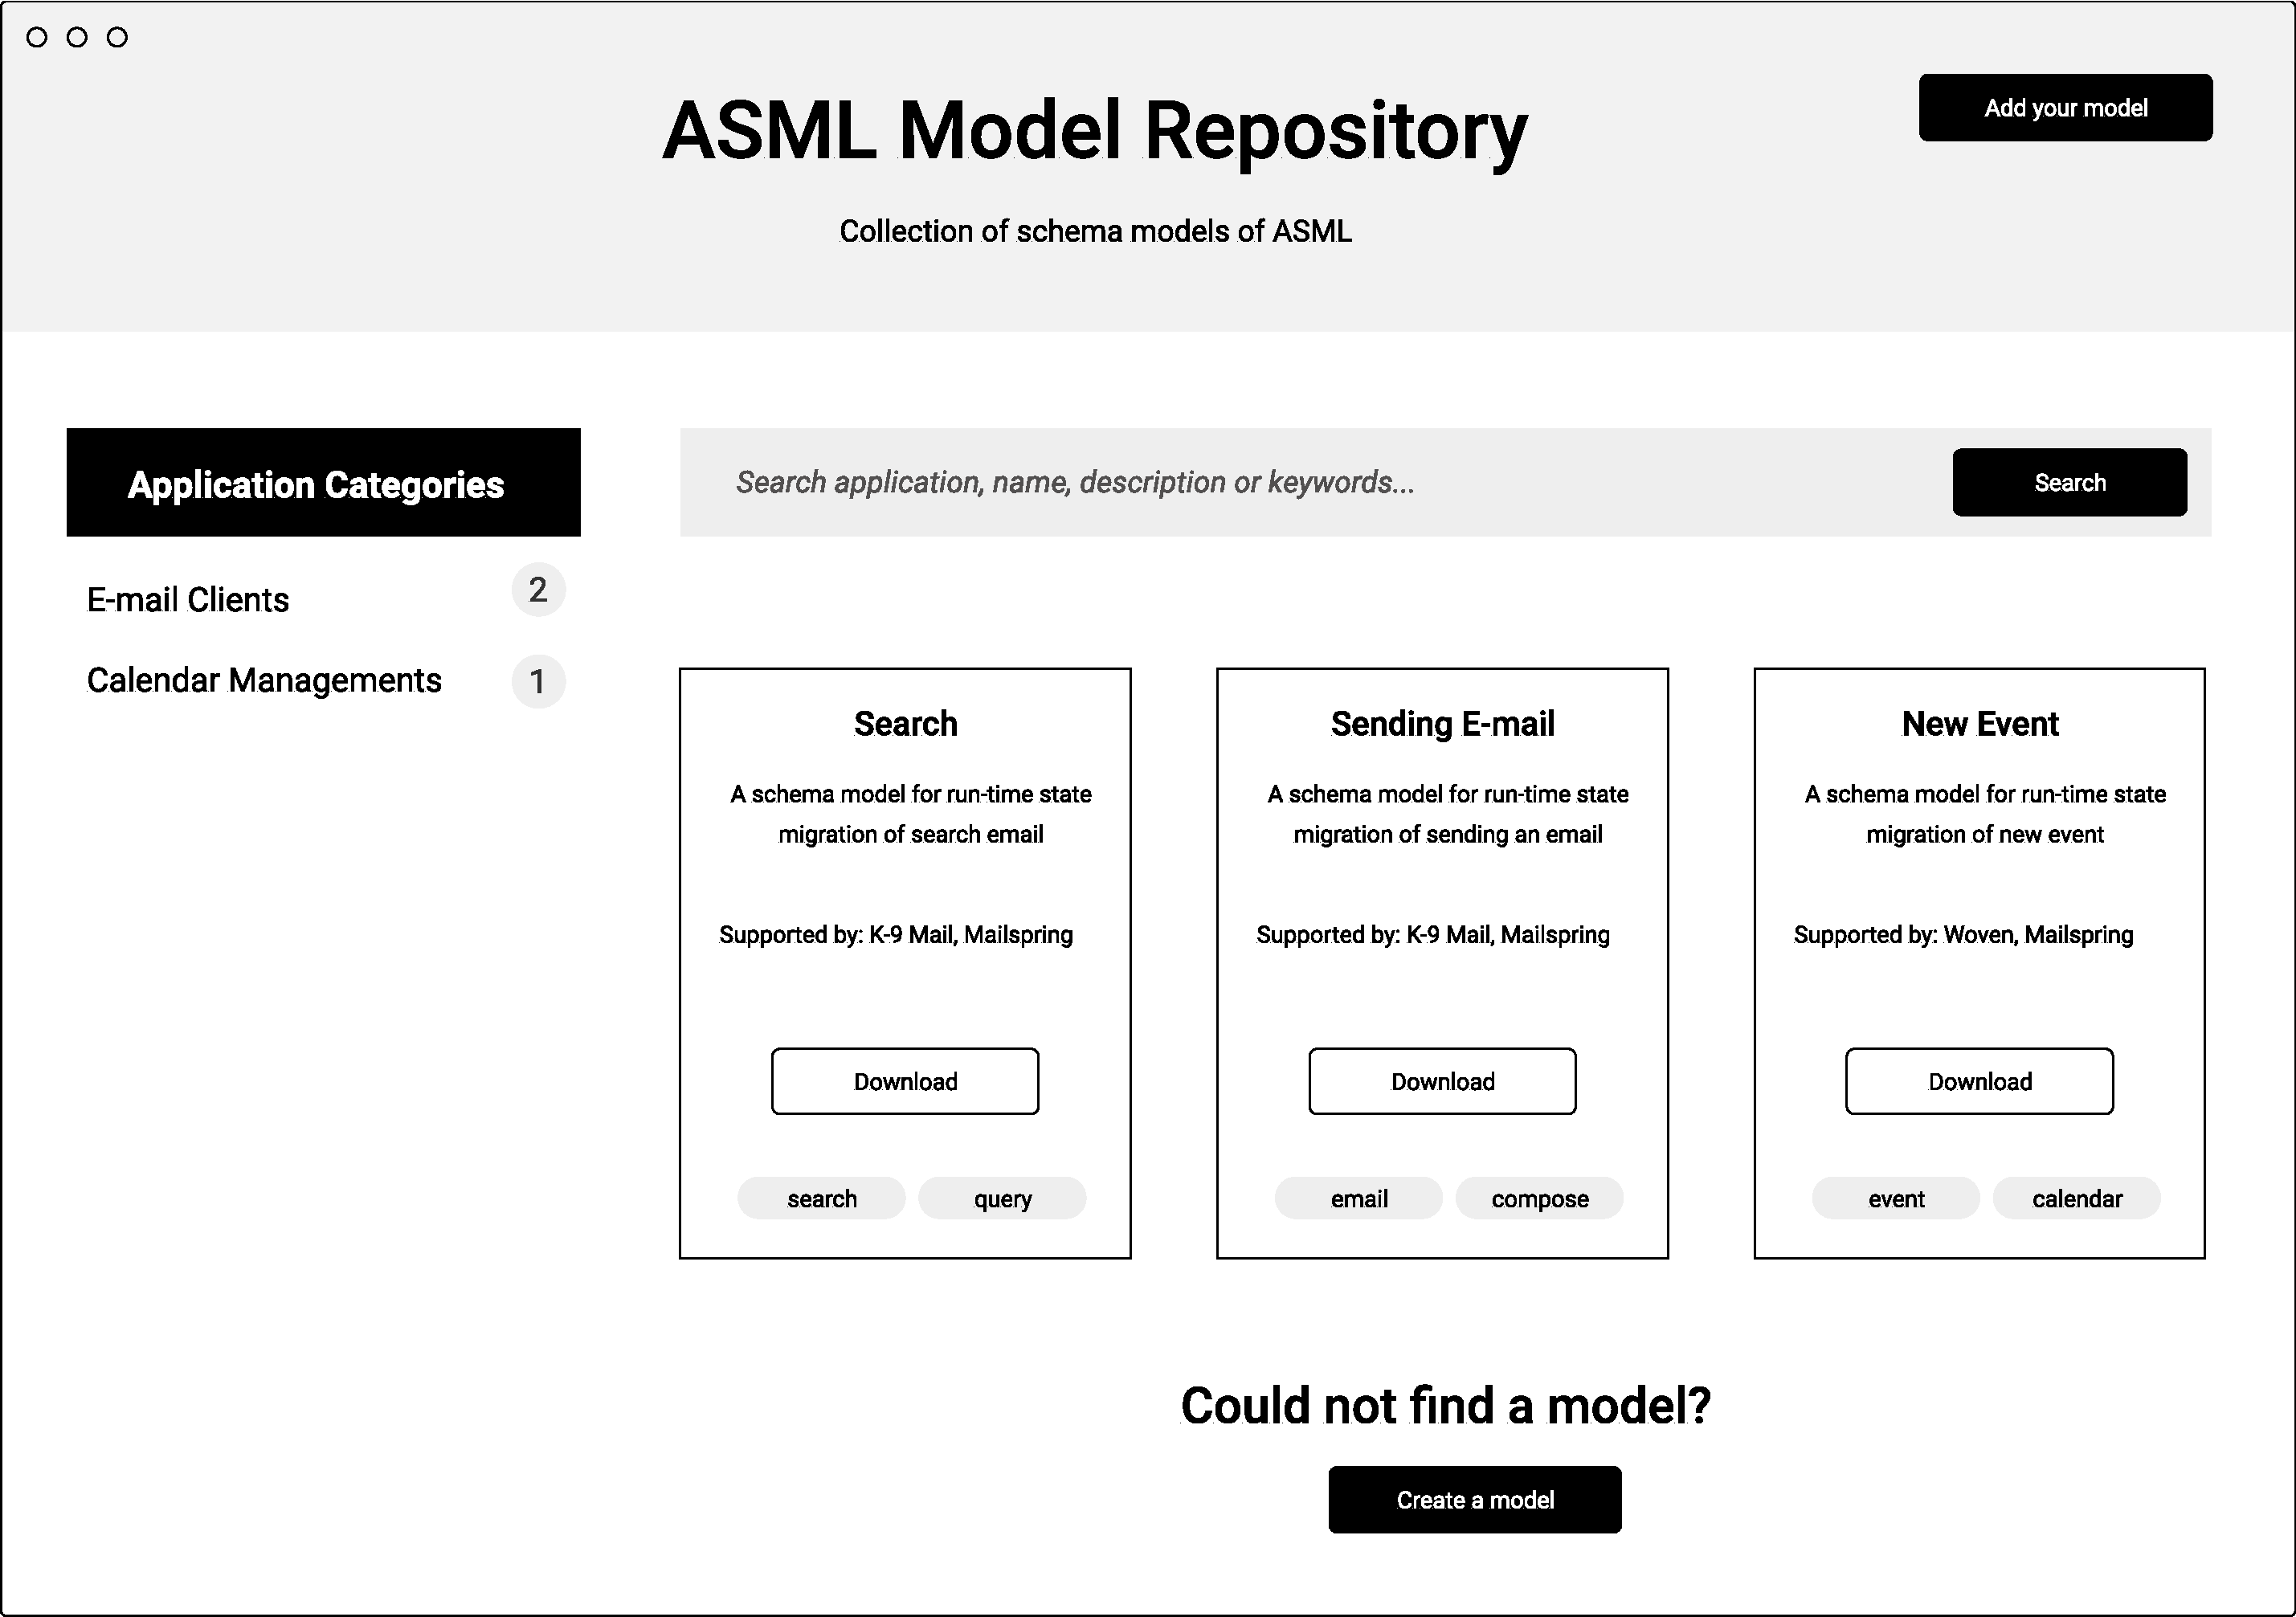
\includegraphics[width=\linewidth]{../figures/model-repo.pdf}
    \centering
    \caption{A wireframe concept for Model Repository}
    \label{fig:model-repo}
\end{figure}
\FloatBarrier